%%%%%%%%%%%%%%%%%%%%%%%%%%%%%%%%%
%
%       EXERCÍCIO
%
%%%%%%%%%%%%%%%%%%%%%%%%%%%%%%%%%

\ifdefstring{\atividade}{prova}{%
    \ifdefstring{\modo}{objetivo}{%
        \renewcommand{\valorquestao}{\ValorQObj\ ponto}
    }{%
        \renewcommand{\valorquestao}{\ValorQDisc\ pontos}
    }%
}%

\begin{exercicioBanco}[\valorquestao]
A figura a seguir ilustra as representações cartesianas das retas $r$ e $s$ de equações $y = x + 3$ e $y = -3x + 27$, respectivamente, com $x$ e $y$ dados em metros. Determine a área, em metros quadrados, do quadrilátero destacado.

\begin{center}
    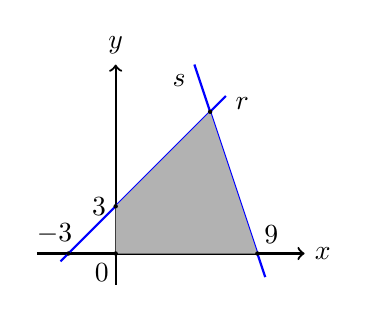
\begin{tikzpicture}[scale=0.2]
        % Eixos
        \draw[->,thick] (-5,0) -- (12,0) node[right] {$x$};
        \draw[->,thick] (0,-2) -- (0,12) node[above] {$y$};

        % Retas
        \draw[domain=-3.5:7, smooth, variable=\x, blue, thick] 
        plot ({\x}, {\x+3});
        
        \draw[domain=5:9.5, smooth, variable=\x, blue, thick] 
        plot ({\x}, {-3*\x+27});

        % Quadrilátero sombreado
        \fill[gray!60]
        (0,0) --
        (0,3) --
        (6,9) --
        (9,0) -- cycle;

        % Marcas no eixo x
        \node[left, above, xshift=-5pt] at (-3,0) {$-3$};
        \node[left, below, xshift=-5pt] at (0,0) {$0$};
        \node[right, above, xshift=5pt] at (9,0) {$9$};

        % Marca no eixo y
        \node[left] at (0,3) {$3$};

        % Identificação das retas
        \node[right] at (7,9.5) {$r$};
        \node[right] at (3,11) {$s$};
        
        % Pontos importantes
        \fill (0,0) circle (4pt);
        \fill (0,3) circle (4pt);
        \fill (6,9) circle (4pt);
        \fill (9,0) circle (4pt);
        \fill (-3,0) circle (4pt);
    \end{tikzpicture}
\end{center}



% Define as alternativas
\newcommand{\alternativas}{%
    \begin{center}
        \begin{tabularx}{\textwidth}{XXXXX}
            (a) \(49,5\) m\(^{2}\). &
            (b) \(49\) m\(^{2}\). &
            (c) \(48,5\) m\(^{2}\). &
            (d) \(48\) m\(^{2}\). &
            (e) \(47,5\) m\(^{2}\).
        \end{tabularx}
    \end{center}
}

% Define a resposta correta
\newcommand{\resposta}{A}

% Lógica condicional para exibição
\ifdefstring{\atividade}{lista}{%
    \alternativas
    \vspace{0.5em}
    
    \noindent\textbf{Resposta:} letra \textbf{\resposta}.
}{%
    \ifdefstring{\modo}{objetivo}{%
        \alternativas
    }{%
        % modo = discursiva → não mostra alternativas
    }
}
\end{exercicioBanco}

